\begin{figure}[H]
\centering
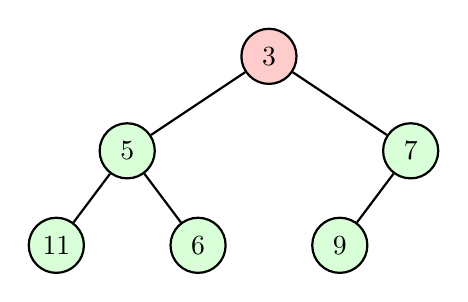
\begin{tikzpicture}[
  vnode/.style={circle, draw, minimum size=7mm, inner sep=0pt, fill=green!15},
  thick, level distance=12mm,
  level 1/.style={sibling distance=36mm},
  level 2/.style={sibling distance=18mm},
  level 3/.style={sibling distance=10mm}
]
  \node[vnode, fill=red!20] (n3) {$3$}
    child { node[vnode] (n5) {$5$}
      child { node[vnode] (n11) {$11$} }
      child { node[vnode] (n6) {$6$} }
    }
    child { node[vnode] (n7) {$7$}
      child { node[vnode] (n9) {$9$} }
      child[missing]
    };
\end{tikzpicture}
\caption{Případ binární minimové haldy. Všimněte si, že každá rodičovská hodnota je menší nebo rovna svým synům a poslední hladina je zaplněna zleva.}
\end{figure}